\section{Całkowanie adaptacyjne}
	\begin{frame}{Całkowanie adaptacyjne}
	\textcolor{blue}{Problem:} $\newline$
      Wzory złożone posiadają węzły równoodległe, jednak
      funkcje mogą mieć w przedziale całkowania różny (przedziałami) przebieg. $\newline$
      $\newline$
      \textbf{Przykładowe przebiegi funkcji:}
      \begin{itemize}
      \item wolnozmienne
      \item oscylacyjne
      \end{itemize}
      $\newline$
      \textcolor{blue}{Rozwiązanie problemu:} $\newline$
      \begin{itemize}
      \item Zastosowanie \textit{procedury rozpoznającej obszar - dobór odpowiedniego kroku!}
      \item Uwzględnienie własności funkcji podcałkowej w obliczeniach
      \end{itemize}
      \end{frame}
%%%%%%%%%%%%%%%%%%%%%%%%%
      \begin{frame}
      \textbf{Dane:}
      \begin{itemize}
      \item $f(x)$ - funkcja podcałkowa
      \item $[a,b]$ - przedział całkowania
      \item $\epsilon$ - dopuszczalny błąd
      \end{itemize}
      \textbf{Idea metody:}$\newline$
      Podział przedziału na fragmenty, dla których zastosowanie jednej z metod klasycznych dało dostatecznie dokładny wynik.
   
      \begin{center}
      		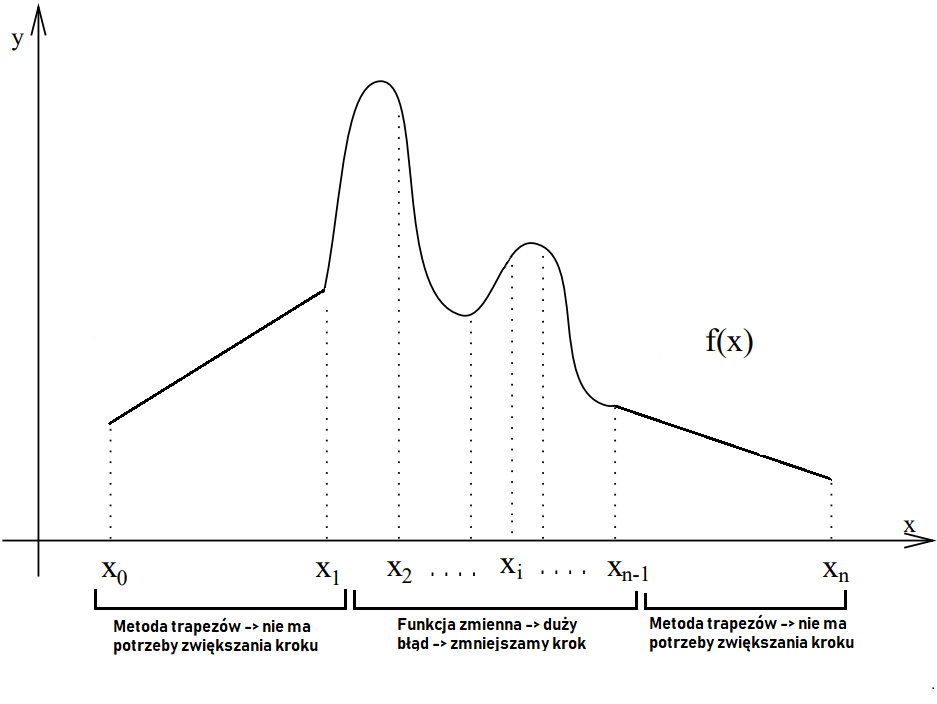
\includegraphics[width=0.6\linewidth]{img/6/image005.png}
      	\end{center}
      \end{frame}
%%%%%%%%%%%%%%%%%%%%%%%%%
      \begin{frame}
      \textbf{Cel:}$\newline$
        Liczymy całkę $\displaystyle \int_{a}^{b}f(x)dx,$\  z dokładnością $\epsilon>0$,\ $f \in C^4[a,b]$
		$\newline$
        1. $m=1$, krok $h=\displaystyle \frac{b-a}{2}$
$\newline$$\newline$
\textbf{Korzystamy ze wzoru Simpsona:}
      
        $$ 
        \int_{a}^{b}f(x)dx=\underbrace{\frac{h}{3}[f(a)+4f(a+h)+f(b)]}_{S(a,b)} - \underbrace{\frac{h^{5}}{90}f^{(4)}(\mu)}_{\alpha} ;\quad \mu\in(a,\ b)
        $$
      \end{frame}
%%%%%%%%%%%%%%%%%%%%%%%%%
      \begin{frame}
      
		2. $m=2$, krok $\displaystyle \frac{h}{2}=\frac{b-a}{4}$ $\newline$
        \scalebox{0.85}{
            $
                \displaystyle \int_{a}^{b}f(x)dx=\frac{h}{6}\underbrace{[f(a)+4f(a+\frac{h}{2})+f(a+h)}_{S(a,\frac{a+b}{2})}+\underbrace{(a+h)+4f(a+\frac{3}{4}h)+f(b)]}_{S(\frac{a+b}{2},b)} - 
            $
        }
        \begin{center}
          \scalebox{0.85}{
            $
            \displaystyle(\frac{h}{2})^{4}\frac{b-a}{180}f^{(4)}(\mu^{\star}) ,\ \mu^{\star}\in(a,\ b)
            $
          }
        \end{center}
        przyjmijmy, że: $f^{(4)}(\mu)\approx f^{(4)}(\mu^{\star})$
		$\newline$$\newline$
        \textbf{Z porównania 1. i 2. :}
        $$
        S(a,b)-\alpha\approx S(a,\ \frac{a+b}{2})+S(\frac{a+b}{2},\ b)-\frac{1}{16}\alpha \quad\Rightarrow
        $$

        $$
        \alpha=\frac{16}{15}[S(a,\ b)-S(a,\ \frac{a+b}{2})-S(\frac{a+b}{2},\ b)]
        $$

	\end{frame}
%%%%%%%%%%%%%%%%%%%%%%%%%
	\begin{frame}
    	Uzyskujemy:
        $\newline$
      \scalebox{0.8}{
          $|\displaystyle \int_{a}^{b}f(x)dx-S(a,\ \frac{a+b}{2})-S(\frac{a+b}{2},\ b)|\approx\frac{1}{15}|s(a,\ b)-S(a,\ \frac{a+b}{2})-S(\frac{a+b}{2},\ b)|$ 
      }
      $\newline$
      \scalebox{0.9}{
      	(lewa strona równania powinna być równa $\epsilon$)
      }
	  $\newline$
      
      Wtedy:
      $$
	      |S(a,\ b)-S(a,\ \frac{a+b}{2})-S(\frac{a+b}{2},\ b)|<15\dot\epsilon \quad(*)
      $$
	\end{frame}
%%%%%%%%%%%%%%%%%%%%%%%%%
	\begin{frame}
    	\textbf{Podsumowanie sposobu postępowania:}$\newline$
        \begin{itemize}
          \item gdy spełnione $(*)$ $\displaystyle \Rightarrow S(a,\ \frac{a+b}{2})+S(\frac{a+b}{2},\ b)\newline$ 
          przybliża całkę $\displaystyle\int_{a}^{b}f(x)dx$ z dokladnością $\epsilon$ $\rightarrow$ STOP
			
          \item nie jest spełnione $(*)$ stosujemy procedurę oceny błędu do przedziałów
$[a,\displaystyle \ \frac{a+b}{2}], [\displaystyle \frac{a+b}{2},\ b]$ w każdym z nich: 	$\displaystyle \epsilon'=\frac{\epsilon}{2}$
          
          \item połowienie podprzedziałów i wyznaczanie $S$
          
          \item ten, na którym odpowiednik $(*)$ nie jest spełniony znów połowimy, pozostałych gotowych nie zmieniamy
            
        \end{itemize}
	\end{frame}
%%%%%%%%%%%%%%%%%%%%%%%%%






















